\documentclass[11pt]{article}\usepackage[margin=0.8in]{geometry}\usepackage[T1]{fontenc}\usepackage{lmodern,tikz,hyperref}\setlength{\parindent}{0pt}\setlength{\parskip}{8pt}\sloppy
\begin{document}\begin{center}{\Large Independent graph Ring word review}\\1 November 2026\end{center}
Seven main declarations, ten producer controls and nine reviewer controls passed fresh isolated Lean replay. Separate axiom readback covers all26 declarations with only standard foundations; two declarations are axiom-free. No discrepancy was found in the stated conditional value semantics.
\begin{center}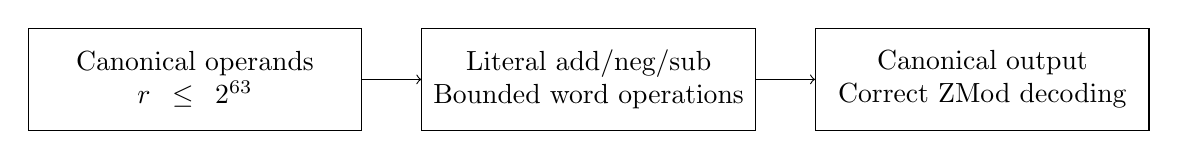
\begin{tikzpicture}[every node/.style={draw,text width=4cm,align=center,minimum height=1.3cm}]
\node(a)at(0,0){Canonical operands\\$r\le2^{63}$};\node(b)at(5,0){Literal add/neg/sub\\Bounded word operations};\node(c)at(10,0){Canonical output\\Correct ZMod decoding};\draw[->](a)--(b);\draw[->](b)--(c);
\end{tikzpicture}\end{center}
\textbf{Source and additive boundary.} Native Ring uses $(a+b)\bmod r$, $(r-a)\bmod r$, and subtraction through negation then addition. Canonical $a,b<r\le2^{63}$ imply $a+b\le2^{64}-2$. The endpoint is valid for the theorem. Ring::new checks primality and $r>2$ but does not enforce this upper bound; constructor success alone cannot establish additive headroom.

\textbf{Literal negation.} The bridge to reduced-input negation is proved using $a\bmod r=a$ under canonicality. It does not silently replace the native expression outside that domain. Negation needs no small-modulus bound beyond positive UInt64 modulus and canonical operand.

\textbf{Wide multiplication.} Both operands widen to128bits before multiplying. The inspected Wide dependency proves the full product fits and remainder lies below $r<2^{64}$, so narrowing is exact. Arbitrary UInt64 operands and any positive modulus are supported by this value model. Retained imported objects were hash-bound, not all rebuilt.

\textbf{Signed branch.} Native i8 sign==1 passes the operand through; every other sign negates it. The theorem uses Int sign restricted to $+1$ or $-1$. The i8 decoding bridge and graph-state sign preservation remain separate. Sign2 is not multiplication by2; sign1 does not canonicalize its input.

\textbf{Independent controls.} Nine kernel controls cover maximum additive headroom, endpoint subtraction, maximal-modulus negation, maximal operand products wide versus narrow, sign2, noncanonical sign1, literal negation underflow and modulus1. Out-of-bound UInt64 examples describe wrapping; Rust overflow-checking builds can panic instead.

\textbf{Remaining scope.} Inverse, prime-constructor correctness, counters/overflow, compiler equivalence and graph potential invariants are not established. Fresh Lean4.34.1 target builds reuse broader Mathlib caches. Private snapshots are hash-bound but not published commits, so full formal-review workflow completion remains false. Full1260-target scope and null cost ratio remain; no scientific execution or measurements occurred.

Source anchor: three\_leads.rs.txt:1492--1534. See REVIEW.md, status.json, axiom-audit.json and exact source/dependency bindings. The first audit parser omitted two axiom-free lines; expected-count validation detected it, and the corrected parser verifies all26.
\end{document}
